\chapter{Variabili aleatorie}
Consideriamo un esperimeno aleatorio, descritto da uno spazio di probabilità $(\Omega, P)$.
\footnote{$\Omega$ = l'insieme di tutti i possibili esiti dell'esperimento, $P$ = probabilità scelta.}
Spesso non siamo interessati a tutti i dettagli dell'esito dell'esperimento, ma oslo a una \emph{quantità, tipicamente numerica, determinata dall'esito dell'esperimento}.
Una tale qunatità è detta \textbf{Variabile Aleatoria}.
\\\\Una Variabile Aleatoria\footnote{detta anche casuale o stocastica.}, è una variabile che può assumere valori diversi in dipendenza da qualche fenomeno aleatorio.
 Il termine "aleatorio" deriva dal latino \textit{alea} (gioco di dadi), ed esprime il
concetto di rischio calcolato.
\begin{center}
    \textit{"alea iacta est"} - "il dado è tratto"
\end{center}

\definizione{
    Una \textbf{Variabile Aleatoria} ha ha due possibili definizioni, una intuitiva e una più matematica:
    \begin{itemize}
        \item Intuitivamente, è una \textbf{quantità che dipende dal "caso"}, ovvero in funzione dell'esito di un esperimento aleatorio.
        \item Matematicamente, è una \textbf{funzione definita sullo spazio campionario}: $X: \Omega \to R$.
    \end{itemize}
}
Ricodiamo che un evento è una affermazione sull'esito dell'esperimento aleatorio, o matematicamente un 
sottoinsieme dello spazio campionario $A \subset \Omega$.

\paragraph{Eventi} Sia $X$ è una variabile aleatoria e $x$ un suo possibile valore:
\\$\{X = x\}$ è un \textbf{Evento} in cui $X$ assume il valore $x$, ovvero:
\[\{X = x\}= \{w \in \Omega: X(w) = x\} \subseteq \Omega\].
Sono possibili eventi anche $\{X \geq x\}$, $\{X \neq x\}$, ...
Ogni variabile aleatoria $X$ determina molti eventi, di cui possiamo calcolare la \textbf{Probabilità}:
\[P(X=x), P(X\geq x), P(X\neq x), ...\]
\esempio{
    Estraggo casualmente una famiglia con due figli/e.
    indichiamo con $X$ il \textbf{numero di figli maschi}.

    Che valori può assumere $X$? Con quali probabilità?
    \[ \Omega = \{ \text{MM,MF,FM,FF} \} \;\;\; P = \text{Probabilità Uniforme} \]
    Allora $X : \omega \to \R$ è definita da:
    \begin{center}
        $X$(MM)=2, $X$(MF)=1, $X$(FM)=1, $X$(FF)=0, 
    \end{center}
    Quindi $X$ assume i valori $X(\Omega)=\{0,1,2\}$, con probabilità: 
    \begin{center}
        $P(X=0)=P(\{$FF$\}) = \frac{1}{4}$, $P(X=2)=P(\{$MM$\}) = \frac{1}{4}$, $P(X=2)=P(\{$MF, FM$\}) = \frac{1}{2}$ 
    \end{center} 
}

\nb{Non bisogna confondere variabili aleatorie ed eventi.}

% DA CAPIRE se questa parte è importante, nel caso da riaggiungere.
% Le variabili aleatorie rappresentano esiti esprimibili numericamente di esperimenti
% ancora da effettuare! Dove per esperimento si intende qualsiasi fenomeno o situazione con sviluppi
% imprevedibili a priori. Essendo imprevedibile a priori il valore assunto da una variabile
% aleatoria, tutto ciò che si può fare è esprimere delle valutazioni di tipo probabilistico sui valori
% che essa assumerà. Per questa ragione ad ogni variabile aleatoria X è associata una funzione che esprime
% in modo chiaro tali valutazioni. 
% \\Se la variabile è discreta si parlerà di \textbf{Densità discreta}.
% \\Se la variabile è continua di parlerà di \textbf{Funzione di ripartizione}.

% \section{Notazione} Con $X_i$ indichiamo la Variabile Aleatoria $X_i: \Omega \rightarrow \mathbb{R}$
% \\ con $x_i$ indichiamo l'osservazione relativa alla V.A $X$

\pagebreak
\section{Variabili Aleatorie Discrete}
\definizione{
    Una variabile aleatoria $X$ (reale) si dice \textbf{discreta} se i valori che può
    assumere sono un insieme finito:
    \[
        X(\Omega) = {x_1, x_2, \dots, x_n} \subseteq  \R
    \]
    Oppure un insieme infinito Numerabile\footnote{Di punti "separati".}:
    \[
        X(\Omega) = {x_1, X_2, \dots } = {x_i} _{i \in \N} \subseteq \R
    \]
}

\subsection{Densità Discreta}
E' concettualmente importante sapere che una Vvariabile Aleatoria $X$ è rappresentata matematicamente da una
una funzione definita sullo spazio campionario $\Omega$ di un esperimento aleatorio.
\[
    X:\Omega \to \R
\]
Allo stesso tempo possiamo pensare a X come a un numero che dipende dal caso.
Se siamo interessati a una v.a. discreta X, spesso non è necessario scrivere lo
spazio campionario $\Omega$ ed esprimere X come funzione, 
ci basta conoscere la \textbf{Densità Discreta}:

\definizione{
    Ad ogni variabile aleatoria discreta $X$ possiamo associare una \textbf{Densità discreta} così definita:
    \[
        p_X(x_i) := P(X = x_i)
    \]
}
Anche detta distribuzione di probabilità, è una funzione che assegna
ad ogni valore possibile di X la probabilità dell'evento $(X = x)$
\subsubsection{Proprietà della densità discreta}
Una densità discreta $p_X$ è una funzione da $\R \in [0,1]$ e gode delle seguenti proprietà:
\begin{itemize}
    \item $p_X(x) = P(X=x) = 0$ Se $x$ non è uno dei valori $x_i$ assunti da $X$.
    \item $p_X(x_i) \geq 0 \forall i$ ($p_X(x_i)\in [0,1]$)
    \item $\sum_{i\geq 1} p_X(x_i) = 1$, perchè gli eventi $\{X=x_i\}$ per $i\geq 1$ sono \textbf{Disgiunti}, ovvero una partizione di $\Omega$.
\end{itemize}
\esempio{
    Riprendiamo l'esempio precedente in cui $X$ era il numero di \textbf{figli maschi} in una famiglia estratta a caso con due figli/e.
    Ricordiamo che $X(\Omega) = \{0,1,2\}$.
    
    Sapendo le probabilità precedenti, quali sono le densità discrete $p_X(x)=P(X=x)$?
    \[
        \implies p_X(0)= \frac{1}{4}, \;\; p_X(1)= \frac{1}{2}, \;\; p_X(2)= \frac{1}{4}
    \]
}

\subsection{Valore Medio}
\definizione{
    Sia X una variabile aleatoria discreta (reale) che assume una quantità finita di valori
    $x_1, x_2, \dots, x_n$. 
    Si definisce \textbf{Valore Medio} di $X$ $E[X]$:
    
    \[
        E[X]:= \sum_{i = 1}^{n} x_i \cdot p_X(x_i) = \sum_{i = 1}^{n} x_i \cdot  P(X= x_i)
    \]
    Ovvero la somma dei valori assunti da $X$ "pesati" con le rispettive probabilità.
}
Il valore medio è anche detto valore atteso, media, espettativa o speranza matematica.
Si indica come $E[X]$ dall'inglese \emph{Expected Value}.

\esempio{
    Riprendendo sempre l'esempio del numero di \textbf{Figli Maschi}:
    \[ X(\Omega) = \{0,1,2\} \text{ con } p_X(0)= p_X(2)=\frac{1}{4}, p_X(1) = \frac{1}{2} \]
    Allora $E[X] = 0 \cdot p_X(0) +  1 \cdot p_X(1) + 2 \cdot p_X(2) = 1$ 
    
    In poche parole se ripetiamo tante volte l'esperimento e ne calcoliamo la media otteniamo
    il valore medio, per esempio il valore medio del numero di figli maschi
    su una coppia con 2 figli è 1, perchè mediamente una coppia con 2 figli ha almeno 1 figlio maschio.

} 
\osservazione{
    Si può notare che il valore medio E[X] non è necessariamente
    uno dei valori $x_i$ assunti da X!
}

A maggior ragione, E[X] non è un valore tipico di X, nè un valore che necessariamente
ci aspettiamo di osservare.
\\ Ma allora qual è l'interpretazione del valore medio $E[X]$? A cosa serve?
Riportiamo l'interpretazione frequentista e quella geometrica di $E{X}$:
\paragraph{Interpretazione frequentista del valore medio}
Supponendo di ripetere l'esperimento aleatorio un numero elevato di volte $N >> 1$
e indicando con $X_1, X_2, \dots, X_n$ le variabili aleatorie che rappresentano X nelle
ripetizioni dell'esperimento si ha con grande probabilità che:
\[
    \frac{X_1 + X_2 + \dots + X_n}{N} \backsimeq  E[X]
\]
Anche detta Legge dei Grandi Numeri.

\paragraph{Interpretazione Geometrica}
Il valore medio $E[X]$ rappresenta il "baricentro" dei valori $x_i$ assunti dalla variabile aleatoria $X$, pesati
con le rispettive probabilità.

\subsubsection{Proprietà del valore medio}
Per ogni variabile aleatoria (reale) $X$ valgono le seguenti proprietà:
\\Per ogni costante $c \in R$
\begin{itemize}
    \item $E[X + c] = E[X] + c$
    \item $E[cX] = c E[X]$
\end{itemize}
Se $X$ e $Y$ sono due variabili aleatorie che dipendono entrambe dallo
stesso esperimento aleatorio, allora:
\begin{itemize}
    \item $E[X+Y] = E[X] + E[Y]$
\end{itemize}
Si dice che il valore medio è un\textbf{ operatore lineare}.
\osservazione{
    Se $Z = X + c$ (oppure $Z=cX$, o $Z = X + Y$) è una variabile aleatoria,
    per calcolare il valore medio $E[Z]$ non c'è bisogno di determinare la densità discreta.
}

\paragraph{Altre importanti proprietà} 
\begin{itemize}
    \item Se $X = c$ (costante) allora $E[X] = E[c] = c$
    \item Se $X >= 0$ allora $E[X] >= 0$
\end{itemize}

\paragraph{Formula di trasferimento} 
\begin{equation}
    E[f(x)] = \sum_{i = 1}^{n} f(x_i)p_X(x_i)
= \sum_{i = 1}^{n}f(x_i)P(X = x_i)
\end{equation}
Valida per ogni funzione $f:R \to R$. In particolare
\begin{equation}
    E[X^2] = \sum_{i = 1}^{n} x_i^2 p_X^{x_i} = \sum_{i = 1}^{n} x_i^2P(X=x_i)
\end{equation}

\paragraph*{Nota per gli esercizi} Queste proprietà servono nel caso in cui ci venga
richiesto di calcolare una nuova media Y in funzione di X, in questo modo applicando
le proprietà non sarà necessario ricalcolare il tutto, ma partendo da Y e applicando
le proprietà di possiamo ricondurre a X e avere già il risultato.

\subsection[Varianza e Deviazione Standard]{Varianza e Deviazione Standard per le Variabili Aleatorie}
Definiamo ora Varianza e Deviazione Standard per le variabili aleatorie:
\definizione{
    Definiamo la Varianza $VAR[X]$ come:
    \[
            VAR[X] := E[(X-\mu)^2] >= 0
    \]
    con $\mu:=E[X]$.
    \\\\E la Deviazione Standard $SD[X]$ come:
    \[ SD[X] := \sqrt{VAR[X]} \]
}
Alternativamente, la deviazione standard può essere definita come:
\[ VAR[X] = E[X^2] - E[X]^2 \]
Questa è una formula più facile da calcolare.

La deviazione standard ha la stessa "unità di misura" di X e fornisce 
una misura della larghezza (o dispersione) dei valori $x_i$ assunti da X rispetto
al valore medio E[X].
\\Valore medio e varianza sono due numeri reali che riassumono
le caratteristiche salienti di una v.a. X (meglio della sua densità discreta).
Sono importanti anche perchè talvolta possono essere calcolati
senza conoscere in dettaglio la densità descrita $p_X$, ma sfruttando le
proprietà di valore medio e varianza.

\subsubsection{Proprietà della varianza}
Per ogni variabile aleatoria (reale) X
\begin{itemize}
    \item $VAR[X+c] = VAR[X]$
    \item $VAR[cX] = c^2 VAR[X]$
\end{itemize}
Per ogni costante reale $c \in R$
\paragraph{Osservazione} Diverse dalle proprietà del valore media!
\\ Varianza = $(SD)^2 \backsimeq $ (larghezza della distribuzione)$^2$
\begin{center}
    Inoltre $X = c \Leftrightarrow VAR[X] = 0$
\end{center}

\paragraph*{Note per gli esercizi} Stesso discordo della media, le proprietà sono super
utili nel caso ci viene richiesto di calcolare una varianza Y in funzione di X e già
calcolata in precedenza.

\subsection{Indipendenza di Variabili Aleatorie}
Siano $X$ e $Y$ due variabili aleatorie, che dipendono entrambe dallo 
stesso esperimento aleatorio. 
\begin{center}
    Quanto vale $VAR[X+Y]$?
\end{center}
La risposta dipende da \textbf{come solo legate $X$ e $Y$!}

\definizione{
    Due Variabili Aleatorie discrete $X$ e $Y$ si dicono \textbf{indipendenti}
    se gli eventi $\{X = x\}$ e $\{Y = y\}$ sono indipendenti, ossia:
    \[
        P(X=x, Y=y) = P(X = x)P(Y = y)
    \]
    Per ogni scelta di $x$ e $y$ tra i valori assunti da $X$ e da $Y$.
}
Intuitivamente conoscere il valore assunto da $X$ non modifica la proabilità dei valori
di $Y$ e viceversa.

Se $X$ e $Y$ sono costruite come funzioni esplicite su uno spazio campionario $\Omega$, 
è possibile mostrare se sono indipendenti.
\\ Molto spesso l'indipendenza è assunta in partenza, ad esempio quando $X$ e $Y$ "non si influenzano". 

\paragraph{Additività della Varianza}
Introduciamo ora un teorema molto importante: quello di additività della varianza.

Se $X$ e $Y$ sono variabili aleatorie \textbf{indipendenti}, allora:
\[
    \var[X+Y] = \var[X] + \var[Y]
\]
Ne segue che la deviazione standard:
\[
    SD[X+Y] = \sqrt{SD[X]^2 + SD[Y]^2}  
\]

\osservazione{
    La relazione di additività della varianza non è affatto scontata e nemmeno intuitiva.
    Infatti la varianza non è lineare, ma la sua somma si comporta linearmente.
}

%%Copiata dagli appunti lezione 6 pagina 3 (con un OCR)
% Se X e Y sono indipendenti e Varie Var Y oh allora
% VARIX Y 28 SATAY RO
% Se la distribuzionedeivalori di X ha larghezza sa 6
% e lo stesso vale per Y la larghezza deivaloridi XYY
% è solo E 6 1,416 non 20
% Questa concentrazione deivalori di X Y è dovuta alla
% indipendenza diXeY
% Il fenomenodiventa ancora piùinteressante quando si sommano
% v ai indipendenti ka ka Xn con N grande vedremo
% la legge dei GRANDINUMERI epoi il teorema limite centrale

\section{Distribuzioni Notevoli Discrete}
Consideriamo una variabile aleatoria $X$, definita nello spazio di probabilità
$(\Omega, P)$ di un certo esperimento aleatorio:
\[
    X:\Omega \rightarrow \mathbb{R} 
\]
Possiamo calcolare la probabilità $P(X \in A)$ per ogni $A \subseteq \mathbb{R}$
(ad esempio per ogni intervallo $A=(a,b)$).
L'insieme di tali probabilità definisce la \textbf{Distriuzione di Probabilità} della Variabile Aleatoria $X$.
\begin{center}
    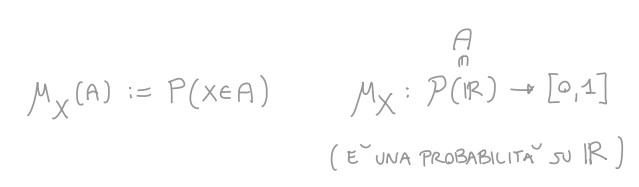
\includegraphics[width=.6\textwidth]{images/funzioneDistribuzione.jpg}
\end{center}

Per Variabili Aleatorie discrete, la distribuzione di $X$ è determinata dalla densità discreta $p_X$:
\[
    P(X \in A) = \sum_{x_i \in A} P(X=x_i) = \sum_{x_i \in A} p_X(x_i)  
\]
Per tale ragione con abuso di notazione, per una v.a. discreta si può chiamare
\textbf{distribuzione} la \textbf{densità discreta}.

Classifichiamo ora le distribuzioni discrete più importanti:

\subsection{Bernoulli}
Si chiama Bernoulli una Variabile Aleatoria $X$ che può \textbf{assumere soltanto i valori 0 e 1} cioè
\[
    X(\Omega) = \{0,1\}
\]
Sia $p:=P(X=1)$, dato che la somma di tutti i valori che può assumere è 1 si ottiene:
\[
    p_X (x) = P(X=x) = 
    \begin{cases}
    p  & \text{ se } x=1\\
    1-p  & \text{ se } x=0
    \end{cases} 
\]
Ovvero:
\[
    \begin{cases}
        P(X=1) = p\\
        P(X=0)= 1-p
    \end{cases}
\]
Quindi $X$ è Bernoulli $\Leftrightarrow$ la sua densità discreta è di questa
forma per un $p \in [0,1]$.
\\ Scriveremo $X \sim \text{Be}(p)$.
\paragraph*{Valore Medio} $E[X] = p$
\paragraph*{Varianza} $\text{Var}[X] = E[X^2] - E[X]^2 = p-p^2 = p(1-p)$

A dispetto della loro semplicità, le variabili aleatorie di bernoulli sono importanti, perchè spesso
vengono utilizzate per costruire variabili aleatorie più complesse.

\subsection{Binomiale}
Consideriamo un esperimento aleatorio costituito da "prove ripetute e indipendenti",
dove ciascua prova può avere due soli esiti "successo" = 1, "insuccesso" = 0, con una
probabilità di successo $p \in [0,1]$ fissata, la stessa per ogni prova.
\esempio{
\begin{itemize}
    \item Lancio ripetutamente una moneta o un dado
    \item Guardo se i figli/e di una coppia sono M o F
    \item estraggo persona da una popolazione molto ampia (successo = elettore del candidato A)
\end{itemize}
}
Siano \begin{itemize}
    \item $n \in \mathbb{N}$ il numero totale di prove.
    \item $p \in [0,1]$ la probabilità di successo in ciascuna prova.
\end{itemize}
Consideriamo quindi la Variabile Aleatoria:
\begin{center}
    $X:=$ numero di "successi" che si verificano nelle $n$ prove.
\end{center} 
La distribuzione di $X$ è detta \textbf{binomiale} di parametri $n$ e $p$ e indicata con $X \sim \text{Bin}(n,p)$
\osservazione{Per $n=1$ ritroviamo Bernoulli: $\text{Bin}(1,p) = \text{Be}(p)$}
Calcoliamo la distribuzione di X. Per costruzione:
\[
    X(\Omega) = \{0,1,2,\dots,n\}
\]
Inoltre la densità discreta è data da:
\begin{equation*}
    p_X (k) = P(X=k) = \binom{n}{k} \cdot p^k \cdot (1-p)^{n-k} \;\;\text{ per } k = 0,1,\dots, n
\end{equation*}
Dove: \begin{itemize}
    \item $\binom{n}{k}$ sono le scelte di quali prove hanno successo,
    ovvero la combinazione di $n$ prove in cui $k$ hanno successo.
    \item $p^k$ è la probabilità di k successi fissati.
    \item $(1-p)^{n-k}$ è la probabilità di $(n-k)$ \underline{in}successi fissati.
\end{itemize}
In definitiva, una variabile aleatoria $X$ è \textbf{binomiale} di parametri $n$ e $p$, $X \sim \text{Bin}(n,p)$,
se ha questa densità discreta.

\paragraph*{Valore Medio} $E[X_i] = np$ 
\paragraph*{Varianza} $Var[X_i]=np(1-p)$

\esempio{
    Riprendendo l'esempio dei figli maschi, sia $X:=$ numero di figli maschi in una coppia con due figli:
    \begin{center}
        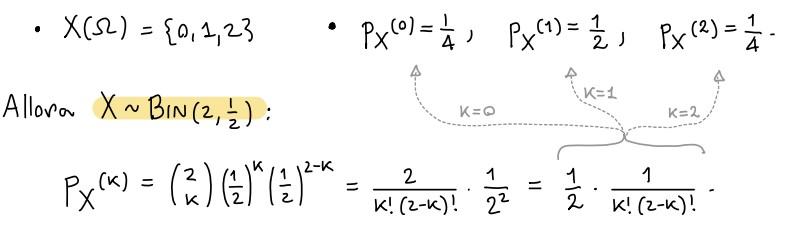
\includegraphics[width=.7\textwidth]{images/figli_maschi_binomiale.jpg}
    \end{center}
    Non è soprendente che $X\sim$Bin$(2,\frac{1}{2})$ perchè possiamo vedere $X$ come il numero
    di "successi" in $n=2$ prover ripetute e indipendenti con probabilità di successo $p=\frac{1}{2}$.
    Infatti
    \[
         X = X_1 + X_2 \;\; \text{dove} \;\; 
        X_i = \begin{cases}
            1 &\text{Se i-esimo figlio è M} \\
            0 & \text{Altrimenti}
        \end{cases}
    \] 
    E le variabili aleatorie $X_1$ e $X_2$ sono Be$(\frac{1}{2})$ indpendenti.
}

\subsection{Poisson}
Una variabile aleatoria \textbf{X si dice Poisson di parametro $\lambda \in (0, \infty)$}, e si
scrive 
\begin{center}
    $X \sim \text{Pois}(\lambda)$
\end{center}
Se $X(\Omega) = \mathbb{N}_0 = {0,1,2,\dots}$ la distribuzione di probabilità è:
\[
    p_X (k) = P(X=k) = e^{-\lambda} \cdot \frac{\lambda^k}{k!} \;\;\; \text{ per } k = 0,1,2,\dots
\]
Si può ottenere una variabile aleatoria di Posson $X \sim \text{Pois}(\lambda)$ come opportuno limite
di una variabile aleatoria binomiale $Y \sim \text{Bin}(n,p)$ quando
\[
    n \rightarrow \infty, p \rightarrow 0 \text{ con } np=\lambda \text{ cioè } p = \frac{\lambda}{n}
\]
\paragraph*{Valore Medio e Varianza}
Se $X \sim \text{Pois}(\lambda)$
\begin{itemize}
    \item $E[X] = \lambda$
    \item $\text{Var}[X] = \lambda$
\end{itemize}

\paragraph*{Poisson in pratica ed Esempi}
Le v.a. di Poisson sono approssimazoni per v.a. che contano il "numero di successi"
quando si considera una grande quantità di prova la cui probabilità di accesso è "piccola".
\\ Qui di seguito alcuni esempi: 
\begin{itemize}
    \item Numero di accessi a una pagina web in un'ora
    \item Numero di nascite in un ospedale in una giornata
    \item Numero di cliente in un ufficio postale in una mattinata
\end{itemize}

\subsection*{Geometrica}
Una v.a. \textbf{X si dice geometrica di parametro $p \in (0,1]$} e si scrive 
\textbf{$X \sim \text{Geo }p$}, se \textbf{$X(\Omega)=\mathbb{N} = {1,2,3,\dots}$} :
\begin{equation*}
    p_X (k) = P(X = k) = p(1-p)^{k-1} \text{per} k=1,2,3,\dots
\end{equation*}
Si può ottenere una v.a. Geo(p) a partire da una successione infinita di prove ripetute
e indipendenti, con probabilità di successo p, e considrando la v.a.
\begin{center}
    T := istante del primo successo
\end{center}
Dove l'istante è il numero della prova.
\\ Ad esempio, indicando con $X_i \sim \text{Be}(p)$ per $i=1,2,3,\dots$ la v.a. che vale 1
se la i-esima prova ha successo, si ha
\begin{equation*}
    P(T=1) = P(X_1 = 1) = p
\end{equation*}
\begin{equation*}
    P(T=2) = P(X_1 = 0, X_2 = 1) = P(X_1 = 0)P(X_2 = 1) = (1-p)p
\end{equation*}
e in generale
\begin{equation*}
    P(T=k) = P(X_1=0, \dots, X_{k-1} = 0, X_k = 1) = (1-p)^{k-1}p
\end{equation*}
\paragraph*{Valore Medio e Varianza} se $X\sim \text{Geo}(p)$
\begin{itemize}
    \item $E[X] = \frac{1}{p}$
    \item $\text{Var}[X] = \frac{1-p}{p^2}$
\end{itemize}
\paragraph*{Note per gli esercizi}
Quando ho un esercizio che riguarda l'estrazione di un elemento n volte, tramite una seria
di prove ripetute e indipendenti, con probabilità di successo p, come lancio di dai o
estrazioni di una pallina colorata con reimmissione allora si tratta di una v.a. con
distribuzione geoemtrica.
% VA Continue

\section{Variabili aleatorie continue}
Esperimento aleatorio $\to$ spazio di probabilità $(\Omega, P)$
\\ Variabile aleatoria $\to$ funzione $X:\Omega \to R$
\\Fin'ora abbiamo studiato v.a. discrete, che assumono un insieme finito oppure
infinito numerabile di valori $X(\Omega) = {x_1, x_2, \dots}$, dove la distribuzione
X è determinata dalla densità discreta:
\begin{equation*}
    p_X^{x_i} = P(X=x_i)
\end{equation*}
\begin{equation}
    P(X \in A) = \sum_{x_i \in A}p_X^{x_i}  
\end{equation}
Consideriamo ora una classe "complementare" di v.a., dette \textbf{assolutamente continue}
che assumono un insieme infinito più che numerabile di valore, come ad es. un intervallo
di R: $[0, 1]$ $[0, +\infty)$ $(-\infty, +\infty)$
\\ Una v.a. è \textbf{assolutamente continua} se la sua distribuzione è determinata
da una funzione $f_x(x)$, a valori positivi, detta densità della v.a. X, nel modo
seguente:
\begin{equation*}
    P(X \in A) = \int_{A}f_x (x) \,dx 
\end{equation*}
In particolare:
\begin{equation*}
    P(X\in[s,t]) = \int_{s}^{t} f_x (x)\,dx 
\end{equation*}
con $-\infty \leq s \leq t \leq +\infty$
\\Area sotto il grafico di $f_x$ tra i punti s e t
\begin{center}
    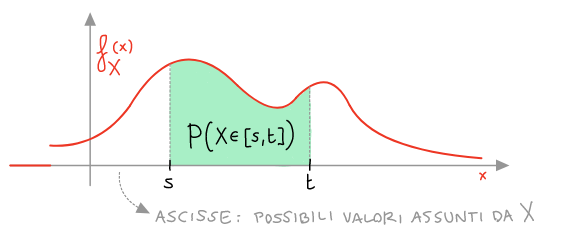
\includegraphics[width=100mm, scale=0.5]{va continue integrale.png}
\end{center}
In altre parole una variabile aleatoria continua può assumere qualunque valore in un
certo intervallo. Esempi di variabile aleatoria continua possono essere il tempo impiegato a
portare a termine un esperimento scientifico o il peso di un individuo.
\\ Ogni v.a. X ha una curva associata. Questa curva, nota come funzione di densità
di probabilità, può essere usata per ottenere le probabilità associate a una v.a.
\\ Visto che \textbf{X assume sempre un valore, otteniamo che l'area totale sottesa dalla curva
deve essere uguale a 1.}
\\ Inoltre visto che l'area sotto il grafico di una funzione di densità di probabilità
tra i punti a e b non varia se gli estremi sono inclusi o esclusi otteniamo che:
\begin{equation*}
    P\{a \leq X \leq b\} = P\{a < X < b \}
\end{equation*}
Questo significa che la probabilità che una variabile aleatoria continua rientri in un
intervallo non cambia se includiamo o no gli estremi.
\\ La curva di densità di probabilità di una v.a. X non scende mai sotto all'asse x ha la
proprietà che l'area delimitata da essa e dall'asse x è sempre uguale a 1.
\\ La curva determina le probabilità di X in questo modo l'area sottesa dalla curva tra i punti a
e b è uguale alla probabilità che X assuma un valore compreso tra a e b.

\subsection*{Analogie tra v.a ass. continua e discreta}
Ci sono analogie formali tra le 2: \begin{itemize}
    \item X ass. continua $P(X \in [s, t]) = \int_{s}^{t} f_x (x) \,dx$ \textbf{Integrale}
    \item X discreta $P(X \in [s, t]) = \sum_{x_i \in [s,t]}p_X (x_i)$ \textbf{Somma}
\end{itemize}
Ma anche importanti differenze!
\\ Se X è assolutamente continua:
\begin{equation*}
    \forall x \in R: P(X=x) = 0
\end{equation*}
\begin{equation*}
    P(X \in [s,t]) = P(X \in (s, t))
\end{equation*}
In particolare: $f_x (x)$ \textbf{NON è} $P(X=x)$, tranne dove $f_x (x) = 0$
\paragraph*{Proprietà} La densità di una v.a. assolutamente continua X è una funzione 
$f_x : R \to R$ (integrabile) tale che: \begin{itemize}
    \item $f_x (x) \geq 0$ $\forall x \in R$
    \item $\int_{-\infty}^{+\infty} f_x (x) \,dx = 1$ Area 
    totale sotto il grafico di $f_x$
\end{itemize}
 \paragraph*{Osservazione} $1 = P(X \in (-\infty, +\infty)) 
 \neq \sum_{x \in (+\infty, -\infty)} P (X = x) = 0$ Dato che $X \in (+\infty, -\infty)$
 è più che numberabile!
 
%Esempio estrazione v.a. uniforme continua
\subsection{Variabile uniforme continua}
Fissiamo un intervallo limitato $[a, b]$ $(-\infty < a < b < -\infty)$.
\\ Una v.a. X si dice uniforme continua in [a, b] e si scrive $X \sim U(a, b)$
se X è ass. cont con densità
\begin{equation*}
    f_x^{x} =
    \begin{cases}
        c \text{ se } x \in [a, b]\\
        0 \text{ se } x \notin [a, b]
    \end{cases} 
\end{equation*}
con $c = \frac{1}{b-a}$
\\ Dato un intervallo $[s, t] \subseteq [a, b]$
\begin{equation*}
    P(X \in [s,t]) = \int_s^t f_x (x) \,dx = 
    \frac{1}{b -a} \int_s^t 1 \,dx = \frac{t-s}{b-a} =
    \frac{\text{Lungh. di } [s,t]}{\text{Lungh. di } [a, b]}
\end{equation*} 
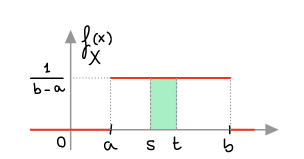
\includegraphics[width=100mm, scale = 0.5]{va unif continua.png}
\paragraph*{Osservazione} Si può mostrare che a partire da una v.a. U(0,1) è possibile
generare una v.a. con distribuzione arbitraria!

\paragraph*{Valori assunti da una V.A assolutamente continua}
\begin{equation*}
    X(\Omega) = {x \in R: f_x(x) > 0S}
\end{equation*}

\paragraph{NB} $f_x(x)$ NON è $P(X=x)$, la densità  di una V.A. Continua non è la densità discreta 
e soprattutto NON è la probabilità di assumere il valore x.

\subsection{Valori assunti da una V.A. assolutamente continua}
La densità di una V.A. assolutamente continua X è una funzione $f_x:\mathbb{R} \rightarrow \mathbb{R}$ (integrabile)
tale che:
\begin{equation*}
    f_x(x) \geq 0 \textrm{ } \forall x \in  \mathbb{R}
\end{equation*}
\begin{equation*}
    \int_{-\infty}^{+\infty} f_x(x)  \,dx = 1
\end{equation*}

Le v.a. assolutamente continue sono necessariamente definite su uno spazio campionario
$\Omega$ infinito più che numerabile.

\begin{equation*}
    X(\Omega) = \{ x \in \mathbb{R} : f_x (x) > 0
\end{equation*}

\section{Valore medio e Varianza di V.A. Assolutamente Continue}
Le definizioni di $E[X]$ e $\text{Var}[X]$ per X ass. continua ricalcano quelle date per
v.a. discrete.
\begin{equation*}
    E[X] = \int_{-\infty}^{+\infty} x f_x(x) \,dx 
\end{equation*}
\subsection*{Varianza}
\begin{equation*}
    E[X^2] = \int_{-\infty}^{+\infty} x^2 f_x(x) \,dx
\end{equation*}
Si definisce $SD[X] := \sqrt[]{\text{Var}[X]}$
\paragraph*{Tutte le proprietà valide nelle v.a. discrete continuano a valere}
In particolare:
\begin{equation*}
    E[X+c] = E[X] + c \qquad E[cX] = cE[X] \qquad E[X+Y] = E[X] + E[Y]
\end{equation*}
\begin{equation*}
    \text{Var}[X+c] = \text{Var}[X] \qquad \text{Var}[cX] = c^2 \text{Var}[X]
\end{equation*}
Se X e y \textbf{sono indipendenti}
\section{V.A. Esponenziale}
Misuro il tempo di emissione X di una particella radioattiva da un atomo, con 
"tempo medio di emissione" $\tau$. Sia $\lambda = \frac{1}{\tau}$.
Descriviamo X con una v.a. assolutamente continua:
\begin{equation*}
    f_X(x) =
    \begin{cases}
        \lambda e^{-\lambda x} \quad \text{se} \, x \geq 0 \\
        0 \quad \text{se} \, x < 0 
    \end{cases}
\end{equation*}
Una v.a. X con tale densità è detta Esponenziale di parametro $\lambda \in (0, \infty)$
e si scrive $X \sim \text{Exp}(\lambda)$.
\\ Per ogni intervallo $[s, t] \subseteq [0, \infty]$:
\begin{equation*}
    P(X \in [s, t]) = \int_{s}^{t} f_x(x)\,dx = \int_{s}^{t} \lambda e^{-lambda x}\,dx=
    [- e^{-\lambda x}]_{s}^{t} =
\end{equation*}
\begin{equation*}
    = e^{-\lambda s} - e^{-\lambda t}
\end{equation*}
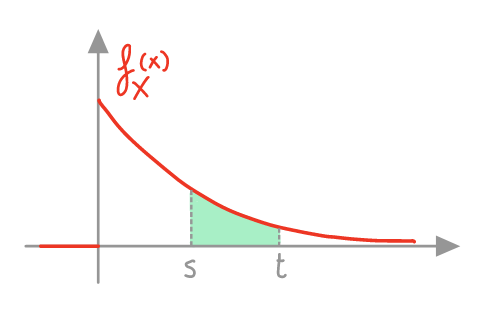
\includegraphics[width=100mm, scale=0.5]{va esponenziale.png}
\section{Funzione di Ripartizione}
Le funzioni di ripartizione ci permettono di capire di che tipo di variabile aleatoria
stiamo parlando.
\begin{equation*}
    F_x (x) = P(X \leq x)
\end{equation*}
A livello probabilistico è la probabilità che X sia minore o uguale a x.
\begin{itemize}
    \item $F_x$ è ben definita per ogni v.a. $X: \Omega \rightarrow \mathbb{R}$, sia che la v.a.
    sia discreta, ass. continua, o nè l'una nè l'altra.
    \item $F_x$ determina la distribuzione della v.a.
    \item $F_x$ è legata alla densità discreta/densità di X
    \begin{equation*}
        F_X(x) = 
        \begin{cases}
        \sum_{x_i \in (- \infty, x]} p_X (x_i) \quad \text{se X è discreta}\\
        \int_{-\infty}^{x} f_x(t)\,dt \quad \text{se X è assolut. continua} 
        \end{cases}
    \end{equation*}
\end{itemize}
La funzione di ripartizione è utile soprattutto per v.a. assolutamente continue, su cui
ci concentreremo nel seguito. Mostriamo comunque un esempio per una v.a. discreta.
\paragraph*{Esempio Bernoulli} Sia $X \sim \text{Be}(p)$ con $p \in (0,1)$.
\begin{equation*}
    X(\Omega) = {0, 1} \qquad p_X{0}=1-p, \qquad p_X(1) = p
\end{equation*}
Allora $F_x(x) = P(X \leq x)$ vale:
\begin{equation*}
    F_X(x) =
    \begin{cases}
        0 \quad \text{se} \quad x < 0 \\
        1-p \quad \text{se} \quad 0 \leq x < 1 \\
        1 \quad se \quad x \leq 1
    \end{cases}
\end{equation*}

\subsection*{Teorema di ripartzione di V.A. Discrete}
\begin{itemize}
    \item X è v.a. discreta $\Leftrightarrow$ $F_x$ è costante a tratti.
    \item Valori assunti{$x_i$} $\Leftrightarrow$ Punti di discontinuità  di $F_x$
    \item Densità discreta $\Leftrightarrow$ Ampiezze dei salti
\end{itemize}
\begin{equation*}
    p_X (x_i) = F_X(x_i) - F_X(X_{\bar{i}})
\end{equation*}
\begin{equation*}
    F_X(x_{\bar{i}}) = \lim_{t \to x_{\bar{i}} F_X(t)}  
\end{equation*}
\subsection*{Funzione di ripartizione di V.A. Assolut. Continue}
X v.a. assolutamente continua $\Leftrightarrow F_X$ è una funzione continua ed
è derivabile a tratti.

\begin{equation}
    \text{Densità} \qquad f_X(x) = (F_X)'(x)
\end{equation}

\section{Variabili aleatorie Normali}
L'ultima classe che vedremo e la più importante, è quella delle variabili aleatorie
normali o Gaussiane.
\\ Una v.a. Z si dice \textbf{Normale Standard} (si scrive $Z \sim N(0,1)$), se è
assolutamente continua con densità:
\begin{equation*}
    f_Z(z)= \frac{1}{\sqrt{2 \pi}} e^{-\frac{z^2}{2}} 
    \quad \forall z \in \mathbb{R}
\end{equation*}
\begin{equation*}
    \rightarrow Z(\Omega) = (-\infty, + \infty)
\end{equation*}
\begin{center}
    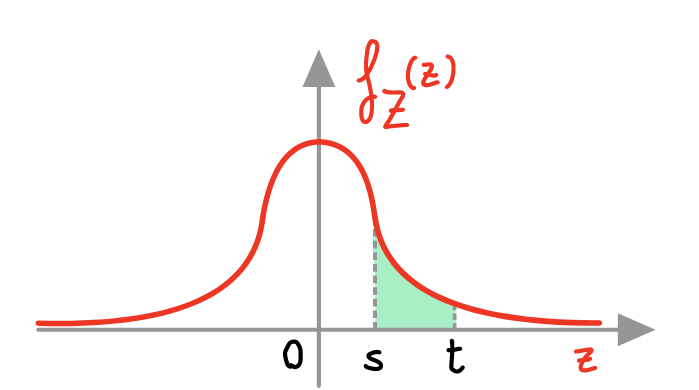
\includegraphics[width=100mm, scale=0.5]{va normale.png}
\end{center}
Come si può notare la forma "a campana" è simmetrica rispetto all'orgine.
\begin{equation}
    \text{"STANDARD"} =
    \begin{cases}
        E[Z] = 0 \\
        \text{Var}[Z] = 1
    \end{cases}
\end{equation}
Dato un intervallo $[s,t] \subseteq \mathbb{R}$
\begin{equation*}
    P(Z\in [s,t]) = \int_{s}^{t} f_z(z)\,dz \qquad 
    \text{(come per ogni v.a. assolutamente continua)}
\end{equation*}
Purtroppo questo integrale non si può calcolare esattamente (la densità $f_Z(z)$
non ammette primitiva esplicita).
\\ Introduciamo la funzione di ripartizione di Z, indicata $\Phi$.
\begin{equation*}
    \Phi(z) = F_Z(z) = P(Z \leq z) = \int_{-\infty}^{z}f_z(t)\,dt
\end{equation*}
Anche questa funzione non di può calcolare esattamente, ma i valori di $\Phi(z)$ per
$z \geq 0$ sono riportati in una tavola.
\\ I valori di $\Phi(z)$ per $z < 0$ si ricavano con la formula
\begin{equation*}
    \Phi(z) = 1 - \Phi(-z)
\end{equation*}
Grazie alla tavola, è come se conoscessimo $\Phi(z) = F_Z(z)$.
Possiamo allora calcolare la probabilità degli intervalli:
\begin{equation*}
    P(Z\in [s,t]) = F_Z(t) - F_Z(s) = \Phi(t) - \Phi(s)
\end{equation*}
Siano ora $\mu \in \mathbb{R}$, $\sigma \in (0, \infty)$.
Una v.a. X si dice \textbf{Normale con media $\mu$ e varianza $\sigma^2$}, si scrive
\textbf{$X \sim N(\mu, \sigma^2)$}, se X è assolutamente continua con
\begin{center}
    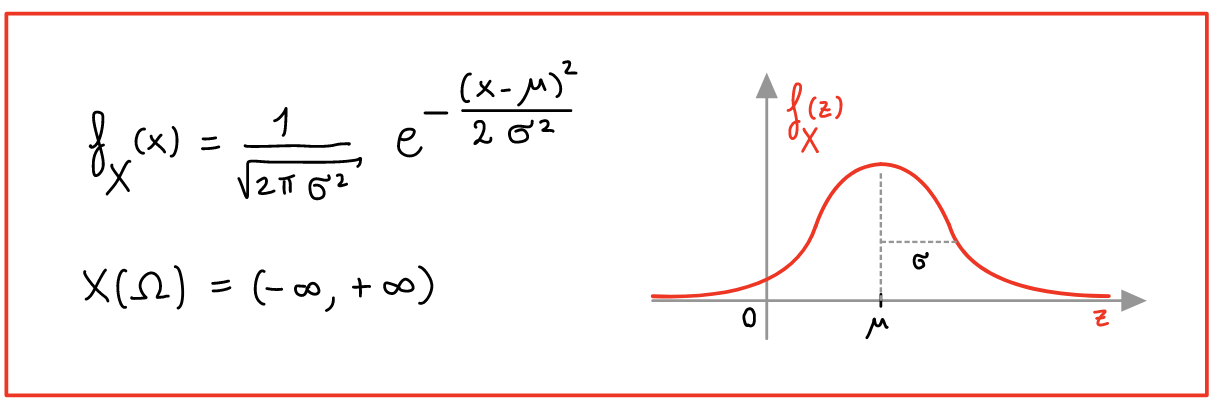
\includegraphics[width=100mm, scale=0.5]{va normale media e var.png}
\end{center}
La densità di $f_X$ di X si ottiene dalla densità di $f_Z$ di $Z \sim N(0,1)$
mediante una traslazione e un riscalamento:
\begin{center}
    $f_X:$ grafico "a campana" centrata in $\mu$, "ampiezza" $\sigma$
\end{center}
Ci si può sempre ricondurre a una v.a. Normale Standard Z:
\begin{equation*}
    X \sim N(\mu, \sigma^2) \rightarrow Z = \frac{X-\mu}{\sigma} \sim N(0,1)
\end{equation*}
\paragraph*{Viceversa}
\begin{equation*}
    Z \sim N(0,1) \rightarrow X = \sigma Z + \mu \sim N(\mu, \sigma^2)
\end{equation*}
Si deduce, in particolare che $\mu$ e $\sigma^2$ sono media e varianza:
\begin{equation*}
    X \sim N(\mu, \sigma^2) \rightarrow E[X] = \mu \quad \text{Var}[X] = \sigma^2
\end{equation*}
Il fatto che ci si può ricondurre a una v.a. normale standard è un caso particolare
della seguente proprietà:
\paragraph*{Teorema} Se X è normale $\rightarrow$ $Y = aX+b$ è normale 
$\forall a \neq 0, b \in \mathbb{R}$
\\ $ X \sim N(\mu, \sigma^2) \rightarrow Y \sim N(a \mu+b, a^2 \sigma^2)$
\begin{itemize}
    \item $E[Y] = aE[X]+b$
    \item $Var[Y] = a^2 Var[X]$
\end{itemize}
\paragraph*{Teorema} X e Y normali indipendenti $\rightarrow X+Y$ è normale.
\begin{equation*}
    X \sim N(\mu_x, \sigma^{2}_x), \, Y \sim N(\mu_y, \sigma^{2}_y)\, \text{indip.}\,
    \rightarrow X+Y \sim N(\mu_x+\mu_y, \sigma^{2}_x + \sigma^{2}_y)
\end{equation*}
\section*{Vettori Aleatori - Non presenti agli esami}
Completare - vedi commento nel codice
%Dato che non è presente nell'esame sarà compilato alla fine, soprattutto se ci sarà
%il tempo
\section{Legge dei grandi numeri}
Completare - vedi commento nel codice
%Dato che è un tema prettamente teorico verrà scritto alla fine della stesura completa
%degli appunti

% Teoremi di convergenza